\chapter{Introduction}
\label{ch:Introduction}

% what are we trying to solve / what is the problem?
% why is it important?

% minimize faulty material
% change contact pressure of steel belt rolls if something's going wrong
% cost reduction
% automatization (IoT, Industry 4.0)

% perform quality checks with sensors
% mechanical parameters can be calculated from magnetic field data
% highly sensitive MEMS gradient magnetometer
% try to predict faulty material in real time

Industry is ever-changing. Especially people working in the information technology branch know that. The latest industry-changing milestone was the rise of the so-called Industry 4.0, which combines regular mechanical processes with moder information and communication technology.

Industry 4.0 is a term that was coined by the german government \cite{Industrie4.0Paper}. It describes the fourth industrial revolution. The first industrial revolution took place around 1800 with the rise of steam and water-powered machines. One century later electricity heralded the start of the second industrial revolution, production lines being on of the biggest milestones. Also division of labour was first practiced. The third industrial revolution occured with the invention of computers, robots and computer automation. The fourth and final one basically just refines the third revolution. This revolution includes the term "cyper-physical systems", which are systems that are controlled by computers, algorithms and sensors. This also means that there has to be some kind of communication between these systems which happens mostly over the internet. Figure \vref{fig:industry40} depicts this sequence of revolutions.

\todo{Cite Industry 4.0 history (https://www.lmis.de/im-wandel-der-zeit-von-industrie-1-0-bis-4-0/)}

\begin{figure}[H]
    \centering
    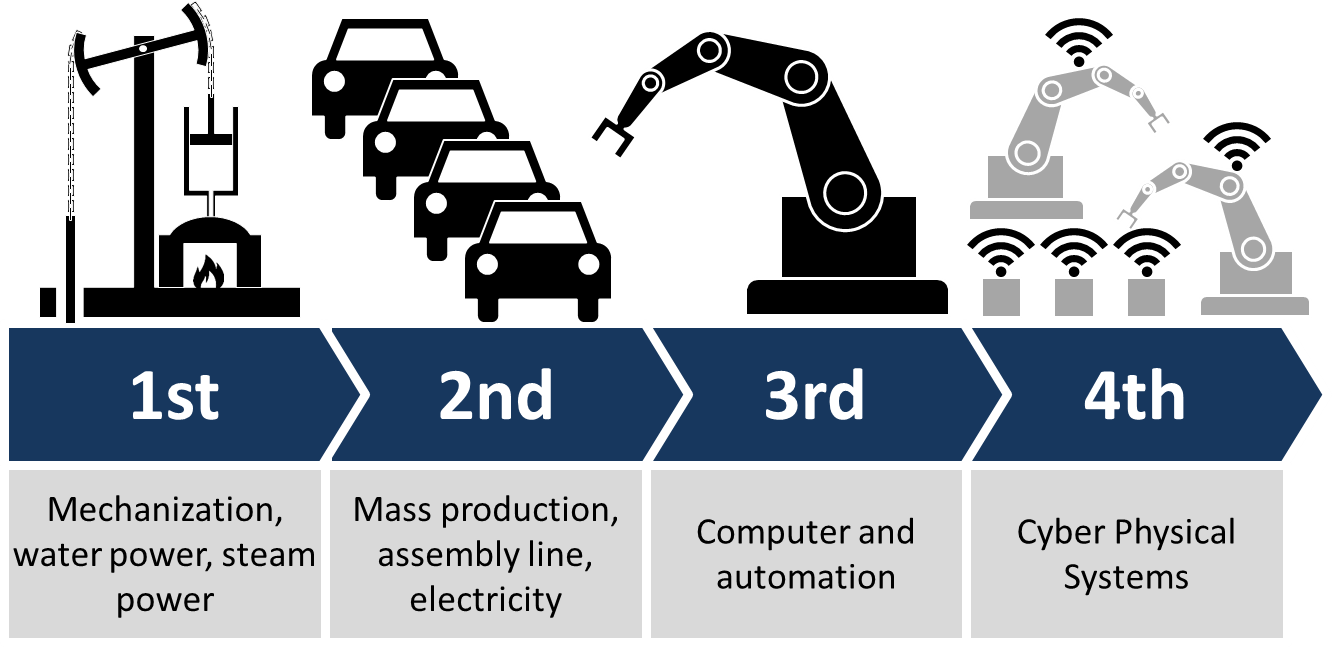
\includegraphics[width=11cm,keepaspectratio]{industry40}
    \caption{The four industrial revolutions that took place over the last centuries. \cite{img:industry4.0}}
    \label{fig:industry40}
\end{figure}

This drastic change means that many companies have to adapt. These adaptions have to be made to keep up with the competing companies.

The invention of a gradient magnetometer that can effectively characterize steel belts the foundation for this diploma thesis were laid.

\todo{cite patent? lol}

\section{Task}

The task of this diploma thesis is to develop a system to read sensor data, process it and visualize the results. Sensor data is continuously read from a highly sensitive MEMS gradient magnetometer. This data is structured as raw binary data and has to be processed by the system. The processed data will also undergoe statistical analysis to predict parameters on the basis of this data. After this processing step the data has to be sent wirelessly to a mobile app. This mobile app acts as the client-side of the system. The app visualizes the sensor data and its predicted parameters. The app should also offer a way of browsing through historical data that was saved prior.

\todo{refactor paragraph, tenses, should}

Server side requirements:

\begin{itemize}
    \item test
\end{itemize}


Client side requirements:

\begin{itemize}
    \item test
\end{itemize}

\section{Current Solutions}

% continuous quality inspection of steel belts
% current solution:
%   produce a certain amount
%   take sample
%   use sample to perform quality checks (stretch tests, ...)
% waste of material / low yield
% time consuming
% not automatable

% real time plotting
% a lot of solutions exist
% little solutions transfer data over network, many assume that sensor is attached to computer
% also no big data volume

\subsection{Existing Solution for Steel Belt Quality Inspection}

The current procedure to inspect the quality of a steel belt is as follows: The first thing that has to be done is to produce a roll of steel belt. To get the quality level of this product, a sample has to be taken from it. There are two samples taken from each steel belt roll, one from the start and one from the beginning. These two samples can now undergo quality inspection procedures. The results from these tests can be used to assess the produced steel belt.

This procedure has a few major disadvantages. Firstly, if the product does not pass the quality tests, the whole steel belt and probably parts of the next belt too can be discarded. The reason for throwing away parts of the belt currently in production is the pressure setting of the steel belt presses. This setting has to be adjusted on the basis of these made quality tests. Time and personnel are also two big disadvantages. These quality tests are not only time consuming but they also require special trained staff for conducting these inspections.

\subsection{Existing Solutions for Handling Sensor Data}

Currently there are a lot of solutions available that can plot sensor data. The majority of these is even free. The one constraint that most of these solutions share is that the sensor has to be directly connected to the computer. As the sensor that is used for this project sends its data over the network, almost all solutions are considered irrelevant. Also some custom features are wanted that these programs do not offer. For example visualizing historical data.

\section{Outline}

% OUTLINE
% short summary of thesis
% explain two phases (I & II)
%   first phase => experimental, learning by doing
%   second phase => 'we know what we were doing', better planned

This diploma thesis is structured into two big parts. These parts can be seen as two phases of implementation. Each phase is completely seperate. The first phase is a more experimental one as both authors were unfamiliar with these types of projects. So some experience had to made. At the end of this phase there was a big cut and it was started from the beginning. The second phase discusses the different approaches and decision that were made starting from this cut. The second phase was not only better planned, but the decisions that were made, were mostly made out of experience from the first phase.
